\documentclass[10pt,landscape]{article}
\usepackage{multicol}
\usepackage{calc}
\usepackage{ifthen}
\usepackage[landscape]{geometry}
\usepackage{verbatim}
\usepackage{graphicx}

\usepackage{color}
\usepackage[usenames,dvipsnames,svgnames,table]{xcolor}
\usepackage{menukeys}

\usepackage{hyperref}
\hypersetup{colorlinks=true}

% Narrow margins
\ifthenelse{\lengthtest { \paperwidth = 11in}}
	{ \geometry{top=.5in,left=.5in,right=.5in,bottom=.5in} }
	{\ifthenelse{ \lengthtest{ \paperwidth = 297mm}}
		{\geometry{top=1cm,left=1cm,right=1cm,bottom=1cm} }
		{\geometry{top=1cm,left=1cm,right=1cm,bottom=1cm} }
	}

% Turn off header and footer
\pagestyle{empty}
 
% Redefine section commands to use less space
\makeatletter
\renewcommand{\section}{\@startsection{section}{1}{0mm}%
                                {-1ex plus -.5ex minus -.2ex}%
                                {0.5ex plus .2ex}%x
                                {\normalfont\large\bfseries\center\color{RoyalBlue}}}
\renewcommand{\subsection}{\@startsection{subsection}{2}{0mm}%
                                {-1explus -.5ex minus -.2ex}%
                                {0.5ex plus .2ex}%
                                {\normalfont\normalsize\bfseries\center\color{Cerulean}}}
\renewcommand{\subsubsection}{\@startsection{subsubsection}{3}{0mm}%
                                {-1ex plus -.5ex minus -.2ex}%
                                {1ex plus .2ex}%
                                {\normalfont\small\bfseries\center\color{ForestGreen}}}
\makeatother

% Highlighted text
\newcommand{\hilight}[1]{\colorbox{yellow}{#1}}

% Don't print section numbers
\setcounter{secnumdepth}{0}


\setlength{\parindent}{0pt}
\setlength{\parskip}{0pt plus 0.5ex}


% -----------------------------------------------------------------------

\begin{document}

\raggedright
\footnotesize
\begin{multicols}{3}

% multicol parameters
% These lengths are set only within the two main columns
%\setlength{\columnseprule}{0.25pt}
\setlength{\premulticols}{1pt}
\setlength{\postmulticols}{1pt}
\setlength{\multicolsep}{1pt}
\setlength{\columnsep}{2pt}

\begin{center}
     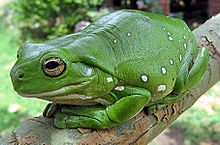
\includegraphics[width=7em]{frog.jpeg}
     \Large{\textbf{\color{WildStrawberry}{Frog Cheat Sheet}}} \\
\end{center}

\section{Section}

\subsection{Subsection}
\subsubsection{Subsubsection}
\begin{tabular}{@{}ll@{} }
\verb!Lorem!        & \hilight{Lorem} ipsum dolor sit amet\\
\verb!ipsum!        & Lorem \hilight{ipsum} dolor sit amet\\
\verb!dolor!      	& Lorem ipsum \hilight{dolor} sit amet\\
\verb!sit!      	& Lorem ipsum dolor \hilight{sit} amet\\
\verb!amet!      	& Lorem ipsum dolor sit \hilight{amet}\\
\end{tabular}

\subsubsection{Another Subsubsection}
	Lorem ipsum dolor sit amet, consectetur adipisicing elit, sed do eiusmod tempor incididunt ut labore et dolore magna aliqua.



\begin{tabular}{@{}ll@{}}
\verb!Lorem!        & Lorem ipsum dolor sit amet\\
\verb!ipsum!        & consectetur adipisicing elit\\
\verb!dolor!      	& sed do eiusmod tempor incididunt ut labore et dolore magna aliqua\\
\verb!sit!      	& Lorem ipsum dolor sit amet\\
\verb!amet!      	& Lorem ipsum dolor sit amet\\
\end{tabular}


\section{Section}

\subsection{Subsection}
\subsubsection{Subsubsection}
\begin{tabular}{@{}ll@{} }
\verb!Lorem!        & \hilight{Lorem} ipsum dolor sit amet\\
\verb!ipsum!        & Lorem \hilight{ipsum} dolor sit amet\\
\verb!dolor!      	& Lorem ipsum \hilight{dolor} sit amet\\
\verb!sit!      	& Lorem ipsum dolor \hilight{sit} amet\\
\verb!amet!      	& Lorem ipsum dolor sit \hilight{amet}\\
\end{tabular}

\subsubsection{Another Subsubsection}
	Lorem ipsum dolor sit amet, consectetur adipisicing elit, sed do eiusmod tempor incididunt ut labore et dolore magna aliqua.



\begin{tabular}{@{}ll@{}}
\verb!Lorem!        & Lorem ipsum dolor sit amet\\
\verb!ipsum!        & consectetur adipisicing elit\\
\verb!dolor!      	& sed do eiusmod tempor incididunt ut labore et dolore magna aliqua\\
\verb!sit!      	& Lorem ipsum dolor sit amet\\
\verb!amet!      	& Lorem ipsum dolor sit amet\\
\end{tabular}


\section{Section}

\subsection{Subsection}
\subsubsection{Subsubsection}
\begin{tabular}{@{}ll@{} }
\verb!Lorem!        & \hilight{Lorem} ipsum dolor sit amet\\
\verb!ipsum!        & Lorem \hilight{ipsum} dolor sit amet\\
\verb!dolor!      	& Lorem ipsum \hilight{dolor} sit amet\\
\verb!sit!      	& Lorem ipsum dolor \hilight{sit} amet\\
\verb!amet!      	& Lorem ipsum dolor sit \hilight{amet}\\
\end{tabular}

\subsubsection{Another Subsubsection}
	Lorem ipsum dolor sit amet, consectetur adipisicing elit, sed do eiusmod tempor incididunt ut labore et dolore magna aliqua.



\begin{tabular}{@{}ll@{}}
\verb!Lorem!        & Lorem ipsum dolor sit amet\\
\verb!ipsum!        & consectetur adipisicing elit\\
\verb!dolor!      	& sed do eiusmod tempor incididunt ut labore et dolore magna aliqua\\
\verb!sit!      	& Lorem ipsum dolor sit amet\\
\verb!amet!      	& Lorem ipsum dolor sit amet\\
\end{tabular}

\begin{center}
\rule{0.3\linewidth}{0.25pt}
\end{center}


\includegraphics[width=6em]{../img/by_nc_sa.eps} This work is licensed under a \href{http://creativecommons.org/licenses/by-nc-sa/3.0/}{Creative Commons Attribution-NonCommercial-ShareAlike 3.0 Unported License}.

{\copyright\ 2012 \href{http://matan.name}{Adam Matan}.}

\begin{tiny}
Sources: 	%\href{http://rayninfo.co.uk/vimtips.html}{Best of Vim Tips},
			%\href{http://people.csail.mit.edu/vgod/vim/vim-cheat-sheet-en.pdf}{Vim Visual Cheat Sheet}
			
StackOverflow.com questions %\href{http://stackoverflow.com/questions/506075/how-do-i-fix-the-indentation-of-an-entire-file-in-vi}	{506075},
							%\href{http://stackoverflow.com/questions/12128678/vim-go-to-beginning-end-of-next-method}				{12128678}

Graphics credits: 	%\href{http://commons.wikimedia.org/wiki/File:Gnome-face-smile.svg}	{Happy icon},
					%\href{http://en.wikipedia.org/wiki/File:Vimlogo.svg}				{Vim Logo},
					\href{http://creativecommons.org/about/downloads}					{Creative Commons License}



Template and general idea based on a \href{http://www.stdout.org/~winston/latex/}{\LaTeX\ template by Winston Chang}.
\end{tiny}




\end{multicols}
\end{document}
